%********************************************%
%*       Generated from PreTeXt source      *%
%*       on 2022-07-27T14:48:44-05:00       *%
%*   A recent stable commit (2020-08-09):   *%
%* 98f21740783f166a773df4dc83cab5293ab63a4a *%
%*                                          *%
%*         https://pretextbook.org          *%
%*                                          *%
%********************************************%
%% We elect to always write snapshot output into <job>.dep file
\RequirePackage{snapshot}
\documentclass[oneside,10pt,]{book}
%% Custom Preamble Entries, early (use latex.preamble.early)
%% Default LaTeX packages
%%   1.  always employed (or nearly so) for some purpose, or
%%   2.  a stylewriter may assume their presence
\usepackage{geometry}
%% Some aspects of the preamble are conditional,
%% the LaTeX engine is one such determinant
\usepackage{ifthen}
%% etoolbox has a variety of modern conveniences
\usepackage{etoolbox}
\usepackage{ifxetex,ifluatex}
%% Raster graphics inclusion
\usepackage{graphicx}
%% Color support, xcolor package
%% Always loaded, for: add/delete text, author tools
%% Here, since tcolorbox loads tikz, and tikz loads xcolor
\PassOptionsToPackage{usenames,dvipsnames,svgnames,table}{xcolor}
\usepackage{xcolor}
%% begin: defined colors, via xcolor package, for styling
%% end: defined colors, via xcolor package, for styling
%% Colored boxes, and much more, though mostly styling
%% skins library provides "enhanced" skin, employing tikzpicture
%% boxes may be configured as "breakable" or "unbreakable"
%% "raster" controls grids of boxes, aka side-by-side
\usepackage{tcolorbox}
\tcbuselibrary{skins}
\tcbuselibrary{breakable}
\tcbuselibrary{raster}
%% We load some "stock" tcolorbox styles that we use a lot
%% Placement here is provisional, there will be some color work also
%% First, black on white, no border, transparent, but no assumption about titles
\tcbset{ bwminimalstyle/.style={size=minimal, boxrule=-0.3pt, frame empty,
colback=white, colbacktitle=white, coltitle=black, opacityfill=0.0} }
%% Second, bold title, run-in to text/paragraph/heading
%% Space afterwards will be controlled by environment,
%% independent of constructions of the tcb title
%% Places \blocktitlefont onto many block titles
\tcbset{ runintitlestyle/.style={fonttitle=\blocktitlefont\upshape\bfseries, attach title to upper} }
%% Spacing prior to each exercise, anywhere
\tcbset{ exercisespacingstyle/.style={before skip={1.5ex plus 0.5ex}} }
%% Spacing prior to each block
\tcbset{ blockspacingstyle/.style={before skip={2.0ex plus 0.5ex}} }
%% xparse allows the construction of more robust commands,
%% this is a necessity for isolating styling and behavior
%% The tcolorbox library of the same name loads the base library
\tcbuselibrary{xparse}
%% The tcolorbox library loads TikZ, its calc package is generally useful,
%% and is necessary for some smaller documents that use partial tcolor boxes
%% See:  https://github.com/PreTeXtBook/pretext/issues/1624
\usetikzlibrary{calc}
%% Hyperref should be here, but likes to be loaded late
%%
%% Inline math delimiters, \(, \), need to be robust
%% 2016-01-31:  latexrelease.sty  supersedes  fixltx2e.sty
%% If  latexrelease.sty  exists, bugfix is in kernel
%% If not, bugfix is in  fixltx2e.sty
%% See:  https://tug.org/TUGboat/tb36-3/tb114ltnews22.pdf
%% and read "Fewer fragile commands" in distribution's  latexchanges.pdf
\IfFileExists{latexrelease.sty}{}{\usepackage{fixltx2e}}
%% Footnote counters and part/chapter counters are manipulated
%% April 2018:  chngcntr  commands now integrated into the kernel,
%% but circa 2018/2019 the package would still try to redefine them,
%% so we need to do the work of loading conditionally for old kernels.
%% From version 1.1a,  chngcntr  should detect defintions made by LaTeX kernel.
\ifdefined\counterwithin
\else
    \usepackage{chngcntr}
\fi
%% Text height identically 9 inches, text width varies on point size
%% See Bringhurst 2.1.1 on measure for recommendations
%% 75 characters per line (count spaces, punctuation) is target
%% which is the upper limit of Bringhurst's recommendations
\geometry{letterpaper,total={340pt,9.0in}}
%% Custom Page Layout Adjustments (use latex.geometry)
%% This LaTeX file may be compiled with pdflatex, xelatex, or lualatex executables
%% LuaTeX is not explicitly supported, but we do accept additions from knowledgeable users
%% The conditional below provides  pdflatex  specific configuration last
%% begin: engine-specific capabilities
\ifthenelse{\boolean{xetex} \or \boolean{luatex}}{%
%% begin: xelatex and lualatex-specific default configuration
\ifxetex\usepackage{xltxtra}\fi
%% realscripts is the only part of xltxtra relevant to lualatex 
\ifluatex\usepackage{realscripts}\fi
%% end:   xelatex and lualatex-specific default configuration
}{
%% begin: pdflatex-specific default configuration
%% We assume a PreTeXt XML source file may have Unicode characters
%% and so we ask LaTeX to parse a UTF-8 encoded file
%% This may work well for accented characters in Western language,
%% but not with Greek, Asian languages, etc.
%% When this is not good enough, switch to the  xelatex  engine
%% where Unicode is better supported (encouraged, even)
\usepackage[utf8]{inputenc}
%% end: pdflatex-specific default configuration
}
%% end:   engine-specific capabilities
%%
%% Fonts.  Conditional on LaTex engine employed.
%% Default Text Font: The Latin Modern fonts are
%% "enhanced versions of the [original TeX] Computer Modern fonts."
%% We use them as the default text font for PreTeXt output.
%% Automatic Font Control
%% Portions of a document, are, or may, be affected by defined commands
%% These are perhaps more flexible when using  xelatex  rather than  pdflatex
%% The following definitions are meant to be re-defined in a style, using \renewcommand
%% They are scoped when employed (in a TeX group), and so should not be defined with an argument
\newcommand{\divisionfont}{\relax}
\newcommand{\blocktitlefont}{\relax}
\newcommand{\contentsfont}{\relax}
\newcommand{\pagefont}{\relax}
\newcommand{\tabularfont}{\relax}
\newcommand{\xreffont}{\relax}
\newcommand{\titlepagefont}{\relax}
%%
\ifthenelse{\boolean{xetex} \or \boolean{luatex}}{%
%% begin: font setup and configuration for use with xelatex
%% Generally, xelatex is necessary for non-Western fonts
%% fontspec package provides extensive control of system fonts,
%% meaning *.otf (OpenType), and apparently *.ttf (TrueType)
%% that live *outside* your TeX/MF tree, and are controlled by your *system*
%% (it is possible that a TeX distribution will place fonts in a system location)
%%
%% The fontspec package is the best vehicle for using different fonts in  xelatex
%% So we load it always, no matter what a publisher or style might want
%%
\usepackage{fontspec}
%%
%% begin: xelatex main font ("font-xelatex-main" template)
%% Latin Modern Roman is the default font for xelatex and so is loaded with a TU encoding
%% *in the format* so we can't touch it, only perhaps adjust it later
%% in one of two ways (then known by NFSS names such as "lmr")
%% (1) via NFSS with font family names such as "lmr" and "lmss"
%% (2) via fontspec with commands like \setmainfont{Latin Modern Roman}
%% The latter requires the font to be known at the system-level by its font name,
%% but will give access to OTF font features through optional arguments
%% https://tex.stackexchange.com/questions/470008/
%% where-and-how-does-fontspec-sty-specify-the-default-font-latin-modern-roman
%% http://tex.stackexchange.com/questions/115321
%% /how-to-optimize-latin-modern-font-with-xelatex
%%
%% end:   xelatex main font ("font-xelatex-main" template)
%% begin: xelatex mono font ("font-xelatex-mono" template)
%% (conditional on non-trivial uses being present in source)
%% end:   xelatex mono font ("font-xelatex-mono" template)
%% begin: xelatex font adjustments ("font-xelatex-style" template)
%% end:   xelatex font adjustments ("font-xelatex-style" template)
%%
%% Extensive support for other languages
\usepackage{polyglossia}
%% Set main/default language based on pretext/@xml:lang value
%% document language code is "en-US", US English
%% usmax variant has extra hypenation
\setmainlanguage[variant=usmax]{english}
%% Enable secondary languages based on discovery of @xml:lang values
%% Enable fonts/scripts based on discovery of @xml:lang values
%% Western languages should be ably covered by Latin Modern Roman
%% end:   font setup and configuration for use with xelatex
}{%
%% begin: font setup and configuration for use with pdflatex
%% begin: pdflatex main font ("font-pdflatex-main" template)
\usepackage{lmodern}
\usepackage[T1]{fontenc}
%% end:   pdflatex main font ("font-pdflatex-main" template)
%% begin: pdflatex mono font ("font-pdflatex-mono" template)
%% (conditional on non-trivial uses being present in source)
%% end:   pdflatex mono font ("font-pdflatex-mono" template)
%% begin: pdflatex font adjustments ("font-pdflatex-style" template)
%% end:   pdflatex font adjustments ("font-pdflatex-style" template)
%% end:   font setup and configuration for use with pdflatex
}
%% Micromanage spacing, etc.  The named "microtype-options"
%% template may be employed to fine-tune package behavior
\usepackage{microtype}
%% Symbols, align environment, commutative diagrams, bracket-matrix
\usepackage{amsmath}
\usepackage{amscd}
\usepackage{amssymb}
%% allow page breaks within display mathematics anywhere
%% level 4 is maximally permissive
%% this is exactly the opposite of AMSmath package philosophy
%% there are per-display, and per-equation options to control this
%% split, aligned, gathered, and alignedat are not affected
\allowdisplaybreaks[4]
%% allow more columns to a matrix
%% can make this even bigger by overriding with  latex.preamble.late  processing option
\setcounter{MaxMatrixCols}{30}
%%
%%
%% Division Titles, and Page Headers/Footers
%% titlesec package, loading "titleps" package cooperatively
%% See code comments about the necessity and purpose of "explicit" option.
%% The "newparttoc" option causes a consistent entry for parts in the ToC 
%% file, but it is only effective if there is a \titleformat for \part.
%% "pagestyles" loads the  titleps  package cooperatively.
\usepackage[explicit, newparttoc, pagestyles]{titlesec}
%% The companion titletoc package for the ToC.
\usepackage{titletoc}
%% Fixes a bug with transition from chapters to appendices in a "book"
%% See generating XSL code for more details about necessity
\newtitlemark{\chaptertitlename}
%% begin: customizations of page styles via the modal "titleps-style" template
%% Designed to use commands from the LaTeX "titleps" package
%% Plain pages should have the same font for page numbers
\renewpagestyle{plain}{%
\setfoot{}{\pagefont\thepage}{}%
}%
%% Single pages as in default LaTeX
\renewpagestyle{headings}{%
\sethead{\pagefont\slshape\MakeUppercase{\ifthechapter{\chaptertitlename\space\thechapter.\space}{}\chaptertitle}}{}{\pagefont\thepage}%
}%
\pagestyle{headings}
%% end: customizations of page styles via the modal "titleps-style" template
%%
%% Create globally-available macros to be provided for style writers
%% These are redefined for each occurence of each division
\newcommand{\divisionnameptx}{\relax}%
\newcommand{\titleptx}{\relax}%
\newcommand{\subtitleptx}{\relax}%
\newcommand{\shortitleptx}{\relax}%
\newcommand{\authorsptx}{\relax}%
\newcommand{\epigraphptx}{\relax}%
%% Create environments for possible occurences of each division
%% Environment for a PTX "chapter" at the level of a LaTeX "chapter"
\NewDocumentEnvironment{chapterptx}{mmmmmm}
{%
\renewcommand{\divisionnameptx}{Chapter}%
\renewcommand{\titleptx}{#1}%
\renewcommand{\subtitleptx}{#2}%
\renewcommand{\shortitleptx}{#3}%
\renewcommand{\authorsptx}{#4}%
\renewcommand{\epigraphptx}{#5}%
\chapter[{#3}]{#1}%
\label{#6}%
}{}%
%% Environment for a PTX "section" at the level of a LaTeX "section"
\NewDocumentEnvironment{sectionptx}{mmmmmm}
{%
\renewcommand{\divisionnameptx}{Section}%
\renewcommand{\titleptx}{#1}%
\renewcommand{\subtitleptx}{#2}%
\renewcommand{\shortitleptx}{#3}%
\renewcommand{\authorsptx}{#4}%
\renewcommand{\epigraphptx}{#5}%
\section[{#3}]{#1}%
\label{#6}%
}{}%
%% Environment for a PTX "subsection" at the level of a LaTeX "subsection"
\NewDocumentEnvironment{subsectionptx}{mmmmmm}
{%
\renewcommand{\divisionnameptx}{Subsection}%
\renewcommand{\titleptx}{#1}%
\renewcommand{\subtitleptx}{#2}%
\renewcommand{\shortitleptx}{#3}%
\renewcommand{\authorsptx}{#4}%
\renewcommand{\epigraphptx}{#5}%
\subsection[{#3}]{#1}%
\label{#6}%
}{}%
%%
%% Styles for six traditional LaTeX divisions
\titleformat{\part}[display]
{\divisionfont\Huge\bfseries\centering}{\divisionnameptx\space\thepart}{30pt}{\Huge#1}
[{\Large\centering\authorsptx}]
\titleformat{\chapter}[display]
{\divisionfont\huge\bfseries}{\divisionnameptx\space\thechapter}{20pt}{\Huge#1}
[{\Large\authorsptx}]
\titleformat{name=\chapter,numberless}[display]
{\divisionfont\huge\bfseries}{}{0pt}{#1}
[{\Large\authorsptx}]
\titlespacing*{\chapter}{0pt}{50pt}{40pt}
\titleformat{\section}[hang]
{\divisionfont\Large\bfseries}{\thesection}{1ex}{#1}
[{\large\authorsptx}]
\titleformat{name=\section,numberless}[block]
{\divisionfont\Large\bfseries}{}{0pt}{#1}
[{\large\authorsptx}]
\titlespacing*{\section}{0pt}{3.5ex plus 1ex minus .2ex}{2.3ex plus .2ex}
\titleformat{\subsection}[hang]
{\divisionfont\large\bfseries}{\thesubsection}{1ex}{#1}
[{\normalsize\authorsptx}]
\titleformat{name=\subsection,numberless}[block]
{\divisionfont\large\bfseries}{}{0pt}{#1}
[{\normalsize\authorsptx}]
\titlespacing*{\subsection}{0pt}{3.25ex plus 1ex minus .2ex}{1.5ex plus .2ex}
\titleformat{\subsubsection}[hang]
{\divisionfont\normalsize\bfseries}{\thesubsubsection}{1em}{#1}
[{\small\authorsptx}]
\titleformat{name=\subsubsection,numberless}[block]
{\divisionfont\normalsize\bfseries}{}{0pt}{#1}
[{\normalsize\authorsptx}]
\titlespacing*{\subsubsection}{0pt}{3.25ex plus 1ex minus .2ex}{1.5ex plus .2ex}
\titleformat{\paragraph}[hang]
{\divisionfont\normalsize\bfseries}{\theparagraph}{1em}{#1}
[{\small\authorsptx}]
\titleformat{name=\paragraph,numberless}[block]
{\divisionfont\normalsize\bfseries}{}{0pt}{#1}
[{\normalsize\authorsptx}]
\titlespacing*{\paragraph}{0pt}{3.25ex plus 1ex minus .2ex}{1.5em}
%%
%% Styles for five traditional LaTeX divisions
\titlecontents{part}%
[0pt]{\contentsmargin{0em}\addvspace{1pc}\contentsfont\bfseries}%
{\Large\thecontentslabel\enspace}{\Large}%
{}%
[\addvspace{.5pc}]%
\titlecontents{chapter}%
[0pt]{\contentsmargin{0em}\addvspace{1pc}\contentsfont\bfseries}%
{\large\thecontentslabel\enspace}{\large}%
{\hfill\bfseries\thecontentspage}%
[\addvspace{.5pc}]%
\dottedcontents{section}[3.8em]{\contentsfont}{2.3em}{1pc}%
\dottedcontents{subsection}[6.1em]{\contentsfont}{3.2em}{1pc}%
\dottedcontents{subsubsection}[9.3em]{\contentsfont}{4.3em}{1pc}%
%%
%% Begin: Semantic Macros
%% To preserve meaning in a LaTeX file
%%
%% \mono macro for content of "c", "cd", "tag", etc elements
%% Also used automatically in other constructions
%% Simply an alias for \texttt
%% Always defined, even if there is no need, or if a specific tt font is not loaded
\newcommand{\mono}[1]{\texttt{#1}}
%%
%% Following semantic macros are only defined here if their
%% use is required only in this specific document
%%
%% Used for inline definitions of terms
\newcommand{\terminology}[1]{\textbf{#1}}
%% Titles of longer works (e.g. books, versus articles)
\newcommand{\pubtitle}[1]{\textsl{#1}}
%% End: Semantic Macros
%% Localize LaTeX supplied names (possibly none)
\renewcommand*{\chaptername}{Chapter}
%% "tcolorbox" environment for a single image, occupying entire \linewidth
%% arguments are left-margin, width, right-margin, as multiples of
%% \linewidth, and are guaranteed to be positive and sum to 1.0
\tcbset{ imagestyle/.style={bwminimalstyle} }
\NewTColorBox{image}{mmm}{imagestyle,left skip=#1\linewidth,width=#2\linewidth}
%% For improved tables
\usepackage{array}
%% Some extra height on each row is desirable, especially with horizontal rules
%% Increment determined experimentally
\setlength{\extrarowheight}{0.2ex}
%% Define variable thickness horizontal rules, full and partial
%% Thicknesses are 0.03, 0.05, 0.08 in the  booktabs  package
\newcommand{\hrulethin}  {\noalign{\hrule height 0.04em}}
\newcommand{\hrulemedium}{\noalign{\hrule height 0.07em}}
\newcommand{\hrulethick} {\noalign{\hrule height 0.11em}}
%% We preserve a copy of the \setlength package before other
%% packages (extpfeil) get a chance to load packages that redefine it
\let\oldsetlength\setlength
\newlength{\Oldarrayrulewidth}
\newcommand{\crulethin}[1]%
{\noalign{\global\oldsetlength{\Oldarrayrulewidth}{\arrayrulewidth}}%
\noalign{\global\oldsetlength{\arrayrulewidth}{0.04em}}\cline{#1}%
\noalign{\global\oldsetlength{\arrayrulewidth}{\Oldarrayrulewidth}}}%
\newcommand{\crulemedium}[1]%
{\noalign{\global\oldsetlength{\Oldarrayrulewidth}{\arrayrulewidth}}%
\noalign{\global\oldsetlength{\arrayrulewidth}{0.07em}}\cline{#1}%
\noalign{\global\oldsetlength{\arrayrulewidth}{\Oldarrayrulewidth}}}
\newcommand{\crulethick}[1]%
{\noalign{\global\oldsetlength{\Oldarrayrulewidth}{\arrayrulewidth}}%
\noalign{\global\oldsetlength{\arrayrulewidth}{0.11em}}\cline{#1}%
\noalign{\global\oldsetlength{\arrayrulewidth}{\Oldarrayrulewidth}}}
%% Single letter column specifiers defined via array package
\newcolumntype{A}{!{\vrule width 0.04em}}
\newcolumntype{B}{!{\vrule width 0.07em}}
\newcolumntype{C}{!{\vrule width 0.11em}}
%% tcolorbox to place tabular outside of a sidebyside
\tcbset{ tabularboxstyle/.style={bwminimalstyle,} }
\newtcolorbox{tabularbox}[3]{tabularboxstyle, left skip=#1\linewidth, width=#2\linewidth,}
%% Footnote Numbering
%% Specified by numbering.footnotes.level
%% Undo counter reset by chapter for a book
\counterwithout{footnote}{chapter}
\counterwithin*{footnote}{section}
%% More flexible list management, esp. for references
%% But also for specifying labels (i.e. custom order) on nested lists
\usepackage{enumitem}
%% hyperref driver does not need to be specified, it will be detected
%% Footnote marks in tcolorbox have broken linking under
%% hyperref, so it is necessary to turn off all linking
%% It *must* be given as a package option, not with \hypersetup
\usepackage[hyperfootnotes=false]{hyperref}
%% configure hyperref's  \href{}{}  and  \nolinkurl  to match listings' inline verbatim
\renewcommand\UrlFont{\small\ttfamily}
%% Hyperlinking active in electronic PDFs, all links without surrounding boxes and blue
\hypersetup{colorlinks=true,linkcolor=blue,citecolor=blue,filecolor=blue,urlcolor=blue}
\hypersetup{pdftitle={Math 1473 - Math for Critical Thinking}}
%% If you manually remove hyperref, leave in this next command
%% This will allow LaTeX compilation, employing this no-op command
\providecommand\phantomsection{}
%% Division Numbering: Chapters, Sections, Subsections, etc
%% Division numbers may be turned off at some level ("depth")
%% A section *always* has depth 1, contrary to us counting from the document root
%% The latex default is 3.  If a larger number is present here, then
%% removing this command may make some cross-references ambiguous
%% The precursor variable $numbering-maxlevel is checked for consistency in the common XSL file
\setcounter{secnumdepth}{3}
%%
%% AMS "proof" environment is no longer used, but we leave previously
%% implemented \qedhere in place, should the LaTeX be recycled
\newcommand{\qedhere}{\relax}
%%
%% A faux tcolorbox whose only purpose is to provide common numbering
%% facilities for most blocks (possibly not projects, 2D displays)
%% Controlled by  numbering.theorems.level  processing parameter
\newtcolorbox[auto counter, number within=section]{block}{}
%%
%% This document is set to number PROJECT-LIKE on a separate numbering scheme
%% So, a faux tcolorbox whose only purpose is to provide this numbering
%% Controlled by  numbering.projects.level  processing parameter
\newtcolorbox[auto counter, number within=section]{project-distinct}{}
%%
%% This document is set to number figure, table, list, listing on a separate numbering scheme
%% So, a faux tcolorbox whose only purpose is to provide this numbering
\newtcolorbox[auto counter]{figure-distinct}{}
%% A faux tcolorbox whose only purpose is to provide common numbering
%% facilities for 2D displays which are subnumbered as part of a "sidebyside"
\makeatletter
\newtcolorbox[auto counter, number within=tcb@cnt@figure-distinct, number freestyle={\noexpand\thetcb@cnt@block(\noexpand\alph{\tcbcounter})}]{subdisplay}{}
\makeatother
%%
%% tcolorbox, with styles, for DEFINITION-LIKE
%%
%% definition: fairly simple numbered block/structure
\tcbset{ definitionstyle/.style={bwminimalstyle, runintitlestyle, blockspacingstyle, after title={\space}, after upper={\space\space\hspace*{\stretch{1}}\(\lozenge\)}, } }
\newtcolorbox[use counter from=block]{definition}[2]{title={{Definition~\thetcbcounter\notblank{#1}{\space\space#1}{}}}, phantomlabel={#2}, breakable, parbox=false, after={\par}, definitionstyle, }
%%
%% tcolorbox, with styles, for EXAMPLE-LIKE
%%
%% example: fairly simple numbered block/structure
\tcbset{ examplestyle/.style={bwminimalstyle, runintitlestyle, blockspacingstyle, after title={\space}, after upper={\space\space\hspace*{\stretch{1}}\(\square\)}, } }
\newtcolorbox[use counter from=block]{example}[2]{title={{Example~\thetcbcounter\notblank{#1}{\space\space#1}{}}}, phantomlabel={#2}, breakable, parbox=false, after={\par}, examplestyle, }
%% question: fairly simple numbered block/structure
\tcbset{ questionstyle/.style={bwminimalstyle, runintitlestyle, blockspacingstyle, after title={\space}, after upper={\space\space\hspace*{\stretch{1}}\(\square\)}, } }
\newtcolorbox[use counter from=block]{question}[2]{title={{Question~\thetcbcounter\notblank{#1}{\space\space#1}{}}}, phantomlabel={#2}, breakable, parbox=false, after={\par}, questionstyle, }
%%
%% xparse environments for introductions and conclusions of divisions
%%
%% introduction: in a structured division
\NewDocumentEnvironment{introduction}{m}
{\notblank{#1}{\noindent\textbf{#1}\space}{}}{\par\medskip}
%%
%% tcolorbox, with styles, for miscellaneous environments
%%
%% assemblage: fairly simple un-numbered block/structure
\tcbset{ assemblagestyle/.style={size=normal, colback=white, colbacktitle=white, coltitle=black, colframe=black, rounded corners, titlerule=0.0pt, center title, fonttitle=\blocktitlefont\bfseries, blockspacingstyle, } }
\newtcolorbox{assemblage}[2]{title={\notblank{#1}{#1}{}}, phantomlabel={#2}, breakable, parbox=false, assemblagestyle}
%% Graphics Preamble Entries
\usepackage{pgfplots}
\usepackage{pgf-pie}
\usepackage{tikz}
	\usetikzlibrary{arrows}
	\usetikzlibrary{arrows.meta}
	\usetikzlibrary{decorations.markings}
	\usetikzlibrary{decorations.pathreplacing}
	\usetikzlibrary{calc}
	\pgfplotsset{compat=1.15}
	\usepgfplotslibrary{fillbetween}
	\usepgfplotslibrary{polar}
%% If tikz has been loaded, replace ampersand with \amp macro
\ifdefined\tikzset
    \tikzset{ampersand replacement = \amp}
\fi
%% extpfeil package for certain extensible arrows,
%% as also provided by MathJax extension of the same name
%% NB: this package loads mtools, which loads calc, which redefines
%%     \setlength, so it can be removed if it seems to be in the 
%%     way and your math does not use:
%%     
%%     \xtwoheadrightarrow, \xtwoheadleftarrow, \xmapsto, \xlongequal, \xtofrom
%%     
%%     we have had to be extra careful with variable thickness
%%     lines in tables, and so also load this package late
\usepackage{extpfeil}
%% Custom Preamble Entries, late (use latex.preamble.late)
%% Begin: Author-provided packages
%% (From  docinfo/latex-preamble/package  elements)
%% End: Author-provided packages
%% Begin: Author-provided macros
%% (From  docinfo/macros  element)
%% Plus three from PTX for XML characters
      \newcommand{\ds}{\displaystyle}
\newcommand{\lrpar}[1]{\left(#1\right)}
\newcommand{\lrbrace}[1]{\left\lbrace #1 \right\rbrace}
\newcommand{\inv}[1]{#1^{-1}}
\newcommand{\R}{\mathbb{R}}
\newcommand{\Z}{\mathbb{Z}}
\newcommand{\dc}{^\circ}
\newcommand{\lt}{<}
\newcommand{\gt}{>}
\newcommand{\amp}{&}
%% End: Author-provided macros
\begin{document}
%% bottom alignment is explicit, since it normally depends on oneside, twoside
\raggedbottom
\frontmatter
%% begin: half-title
\thispagestyle{empty}
{\titlepagefont\centering
\vspace*{0.28\textheight}
{\Huge Math 1473 - Math for Critical Thinking}\\}
\clearpage
%% end:   half-title
%% begin: title page
%% Inspired by Peter Wilson's "titleDB" in "titlepages" CTAN package
\thispagestyle{empty}
{\titlepagefont\centering
\vspace*{0.14\textheight}
%% Target for xref to top-level element is ToC
\addtocontents{toc}{\protect\hypertarget{x:book:math1473}{}}
{\Huge Math 1473 - Math for Critical Thinking}\\[3\baselineskip]
{\Large Cory Wilson}\\[0.5\baselineskip]
{\Large University of Oklahoma}\\[3\baselineskip]
{\Large July 27, 2022}\\}
\clearpage
%% end:   title page
%% begin: copyright-page
\thispagestyle{empty}
\hypertarget{x:colophon:colophon}{}\vspace*{\stretch{2}}
\noindent\textcopyright{}2022\quad{}Cory Wilson\\[0.5\baselineskip]
This work is licensed under the Creative Commons Attribution-ShareAlike 4.0 International License. To view a copy of this license, visit \href{http://creativecommons.org/licenses/by-sa/4.0/}{http:\slash{}\slash{}creativecommons.org\slash{}licenses\slash{}by-sa\slash{}4.0\slash{}}\footnote{\nolinkurl{http://creativecommons.org/licenses/by-sa/4.0/}\label{g:fn:idp1505389848}}.\par\medskip
\vspace*{\stretch{1}}
\null\clearpage
%% end:   copyright-page
%% begin: table of contents
%% Adjust Table of Contents
\setcounter{tocdepth}{1}
\renewcommand*\contentsname{Contents}
\tableofcontents
%% end:   table of contents
\mainmatter
%
%
\typeout{************************************************}
\typeout{Chapter 1 Representing Data}
\typeout{************************************************}
%
\begin{chapterptx}{Representing Data}{}{Representing Data}{}{}{x:chapter:data}
\begin{introduction}{}%
This unit focuses on different ways to represent data.  We will specifically investigate representing data in tables, representing data graphically, and ways of interpreting represented data.%
\par
Directly below are links to quickly navigate to individual sections.%
\end{introduction}%
%
%
\typeout{************************************************}
\typeout{Section 1.1 Qualitative Data}
\typeout{************************************************}
%
\begin{sectionptx}{Qualitative Data}{}{Qualitative Data}{}{}{x:section:data-qual}
%
%
\typeout{************************************************}
\typeout{Subsection 1.1.1 Qualitative and Quantitative Data}
\typeout{************************************************}
%
\begin{subsectionptx}{Qualitative and Quantitative Data}{}{Qualitative and Quantitative Data}{}{}{x:subsection:data-rep-qualquant}
Data is all around us, and informs much of how our lives run.  Let's focus on two specific types of data, \terminology{qualitative data} and \terminology{qualitative data}.%
\begin{definition}{}{x:definition:qualquantdata}%
\terminology{Qualitative data} is data which describes qualities or characteristics.  Sometimes qualitative data is called \terminology{categorical data}.%
\par
\terminology{Quantitative data} is data which is represented using numbers.%
\index{Qualitative data}%
\index{Quantitative data}%
\index{Categorical data}%
\end{definition}
\begin{example}{}{g:example:idp1542515848}%
Classify the following data from members of our class as qualitative or quantitative.  Give a brief explanation for the answer. %
\begin{enumerate}[label=\alph*]
\item{}Color of hair%
\item{}Political affiliation%
\item{}Height%
\item{}Classification by credit hours%
\item{}Number of hours taken this semester%
\end{enumerate}
\par\smallskip%
\noindent\hypertarget{g:solution:idp1542518152}{}%
\begin{enumerate}[label=\alph*]
\item{}Quantiative - color is a quality%
\item{}Quantitative - the description is verbal\slash{}a quality%
\item{}Qualitative - the height will be given numerically%
\item{}Quantitative - even though we can look at year in school, classification ("freshman", "junior", etc.) is verbal%
\item{}Quantitative - credit hours are numerical%
\end{enumerate}
%
\end{example}
\begin{example}{}{g:example:idp1542530056}%
Come up with three sets of quantitative data and three sets of qualitative data.  These should be different than the previous example!%
\par\smallskip%
\noindent\textbf{\blocktitlefont Solution}.\hypertarget{g:solution:idp1542526984}{}\quad{}Answers vary%
\end{example}
\end{subsectionptx}
%
%
\typeout{************************************************}
\typeout{Subsection 1.1.2 Representing Qualitative Data}
\typeout{************************************************}
%
\begin{subsectionptx}{Representing Qualitative Data}{}{Representing Qualitative Data}{}{}{x:subsection:data-rep-frequency}
When data is collected, we need a way to communicate the information effectively.%
\par
One way of communicating qualitative information is by using a \terminology{frequency distribution}.%
\begin{definition}{}{x:definition:frequencydist}%
A \terminology{frequency distribution} is a two-column table which collects the number of times a category appears in a set of data.%
\index{Frequency distribution}%
\end{definition}
\begin{example}{}{g:example:idp1542529544}%
A store employee is doing an inventory of items near the register.  They found 51 bags of chips, 62 candy bars, 47 bags of candy, 121 packs of gum, 16 bags of nuts, 20 soft drinks, and 20 bottles of water.  Create a frequency table to display the result of the inventory.\par\smallskip%
\noindent\textbf{\blocktitlefont Solution}.\hypertarget{g:solution:idp1542528264}{}\quad{}\begin{center}%
{\tabularfont%
\begin{tabular}{ll}
Item&Frequency\tabularnewline[0pt]
Chips&51\tabularnewline[0pt]
Candy Bars&62\tabularnewline[0pt]
Candy Bags&47\tabularnewline[0pt]
Gum&121\tabularnewline[0pt]
Nuts&16\tabularnewline[0pt]
Soft Drinks&20\tabularnewline[0pt]
Water&20
\end{tabular}
}%
\end{center}%
%
\end{example}
\begin{example}{}{g:example:idp1542538760}%
Find out the state (or country) of birth of the portion of the class your instructor specifies.  Once you've collected the data, create a frequency table for the data.%
\par\smallskip%
\noindent\textbf{\blocktitlefont Solution}.\hypertarget{g:solution:idp1542535432}{}\quad{}Answers vary%
\end{example}
We can also graphically represent qualitative data.  This is often done using a \terminology{bar graph}.%
\begin{definition}{}{x:definition:bargraph}%
A \terminology{bar graph} is a graph that represents category frequencies with a bar whose length is equal to the frequency.%
\index{Bar Graph}%
\end{definition}
\begin{example}{}{g:example:idp1542534536}%
Create a bar graph for the data from Example 1.1.2.  For convenience, here is the data again: A store employee is doing an inventory of items near the register.  They found 51 bags of chips, 62 candy bars, 47 bags of candy, 121 packs of gum, 16 bags of nuts, 20 soft drinks, and 20 bottles of water.%
\par\smallskip%
\noindent\textbf{\blocktitlefont Solution}.\hypertarget{g:solution:idp1542532744}{}\quad{}There's a lot of variation in this, but the graph should look something like this.%
\par
\begin{image}{0}{1}{0}%
\resizebox{\linewidth}{!}{%
\begin{tikzpicture}
    \begin{axis}[
        title = Inventory Results,
        ybar,
        bar width = 0.5cm,
        symbolic x coords = {Chips, Bars, Bags, Gum, Nuts, Sodas, Water},
    ]
    \addplot coordinates {(Chips, 51) (Bars, 62) (Bags, 47) (Gum, 121) (Nuts, 16) (Sodas, 20) (Water, 20)};
    \end{axis}
\end{tikzpicture}
}%
\end{image}%
%
\end{example}
\begin{assemblage}{Bar Graph Features.}{g:assemblage:idp1542541960}%
Bar graphs should have the following features:%
\par
%
\begin{itemize}[label=\textbullet]
\item{}Vertical axis with label%
\item{}Horizontal axis with labels%
\item{}A consistent scale on the vertical axis%
\item{}A descriptive title%
\end{itemize}
%
\end{assemblage}
\begin{assemblage}{Note.}{g:assemblage:idp1542539912}%
Bar graphs can be oriented vertically (like we just did) or horizontally.  If they are oriented horizontally, the vertical and horizontal information flips, but all other features will remain the same.%
\end{assemblage}
\begin{example}{}{g:example:idp1542542856}%
Now create a bar graph for the data you collected about home states\slash{}countries.  Be sure to include the features listed above!%
\par\smallskip%
\noindent\textbf{\blocktitlefont Solution}.\hypertarget{g:solution:idp1542547336}{}\quad{}Answers vary%
\end{example}
A special type of bar graph is called a \terminology{Pareto chart}.%
\begin{definition}{}{x:definition:pareto}%
A \terminology{Pareto chart} is a bar graph whose bars are ordered from highest to lowest frequency.%
\index{Pareto chart}%
\end{definition}
\begin{example}{}{g:example:idp1542543496}%
A recent Math 1473 class had 15 freshmen, 3 sophomores, 10 juniors, and 8 seniors.  Create the Pareto chart for the data.%
\par\smallskip%
\noindent\textbf{\blocktitlefont Solution}.\hypertarget{g:solution:idp1542555528}{}\quad{}As before, the bar chart should look something like this.%
\par
\begin{image}{0}{1}{0}%
\resizebox{\linewidth}{!}{%
\begin{tikzpicture}
    \begin{axis}[
            title = Class Makeup,
            ybar,
            nodes near coords,
            bar width = 0.5cm,
            symbolic x coords = {Fresh, Jun, Sen, Soph},
            xtick ={Fresh, Jun, Sen, Soph},
        ]
        \addplot coordinates {(Fresh, 15) (Jun, 10) (Sen, 8) (Soph, 3) };
    \end{axis}
\end{tikzpicture}
}%
\end{image}%
%
\end{example}
Sometimes it is helpful to more than one qualtitative variable on a graph.  This can be accomplished by creating a \terminology{side-by-side bar graph} or a \terminology{stacked bar graph}.%
\begin{definition}{}{x:definition:sbsbar}%
A \terminology{side-by-side bar graph} is a bar graph which shows two or more bars next to each other%
\index{Side-by-side Bar Graph}%
\end{definition}
\begin{example}{}{g:example:idp1542555144}%
The 2020 US Census gave the following data about racial identities in the top three most populous cities in Oklahoma: \begin{center}%
{\tabularfont%
\begin{tabular}{llll}
Race&Oklahoma City&Tulsa&Norman\tabularnewline[0pt]
White only&364,706&214,012&89,283\tabularnewline[0pt]
Black\slash{}African American only&95,634&61,526&6,398\tabularnewline[0pt]
Asian only&31,510&14,352&5,083
\end{tabular}
}%
\end{center}%
%
\par
Create a side-by-side bar graph to display the data.%
\par\smallskip%
\noindent\textbf{\blocktitlefont Solution}.\hypertarget{g:solution:idp1542560776}{}\quad{}The scale on this is hard to get right, but it's something like this.%
\par
\begin{image}{0}{1}{0}%
\resizebox{\linewidth}{!}{%
\begin{tikzpicture}
    \begin{axis}[
        title = Racial Makeup of Oklahoma's 3 Largest Cities (in thousands),
        ybar,
        nodes near coords,
        bar width = 0.5cm,
        symbolic x coords = {OKC, Tulsa, Norman},
        xtick = {OKC, Tulsa, Norman},
        enlarge x limits = 0.25,
        ymin = 0,
        legend cell align = left,
        ]
        
        \addplot coordinates {(OKC, 364.706) (Tulsa, 214.012) (Norman, 89.283)}; %whites
        \addplot coordinates {(OKC, 95.634) (Tulsa, 61.526) (Norman, 6.398)}; %blacks
        \addplot coordinates {(OKC, 31.510) (Tulsa, 14.352) (Norman, 5.083)}; %asians
        \legend{White, Black, Asian};
    \end{axis}
\end{tikzpicture}
}%
\end{image}%
%
\end{example}
Note that in this example, we needed to include a \terminology{legend} in order to identify what each bar was telling us.%
\begin{definition}{}{x:definition:stackedbar}%
A \terminology{stacked bar graph} is a bar graph in which bars are stacked on top of each other to show relative size.%
\index{Stacked Bar Graph}%
\end{definition}
\begin{example}{}{g:example:idp1542563720}%
Use a stacked bar graph to display the Census data from Example 1.1.13.  Here it is again:%
\par
The 2020 US Census gave the following data about racial identities in the top three most populous cities in Oklahoma: \begin{center}%
{\tabularfont%
\begin{tabular}{llll}
Race&Oklahoma City&Tulsa&Norman\tabularnewline[0pt]
White only&364,706&214,012&89,283\tabularnewline[0pt]
Black\slash{}African American only&95,634&61,526&6,398\tabularnewline[0pt]
Asian only&31,510&14,352&5,083
\end{tabular}
}%
\end{center}%
%
\par\smallskip%
\noindent\textbf{\blocktitlefont Solution}.\hypertarget{g:solution:idp1542570376}{}\quad{}\begin{image}{0}{1}{0}%
\resizebox{\linewidth}{!}{%
\begin{tikzpicture}
    \begin{axis}[
        title = Racial Makeup of Oklahoma's 3 Largest Cities (in thousands),
        ybar stacked,
        bar width = 2cm,
        nodes near coords,
        symbolic x coords = {OKC, Tulsa, Norman},
        xtick = {OKC, Tulsa, Norman},
        enlarge x limits = 0.25,
        ymin = 0,
        legend cell align = left,
        ]
        
        \addplot+[ybar] plot coordinates {(OKC, 364.706) (Tulsa, 214.012) (Norman, 89.283)}; %whites
        \addplot+[ybar] plot coordinates {(OKC, 95.634) (Tulsa, 61.526) (Norman, 6.398)}; %blacks
        \addplot+[ybar] plot coordinates {(OKC, 31.510) (Tulsa, 14.352) (Norman, 5.083)}; %asians
        \legend{White, Black, Asian};
    \end{axis}
\end{tikzpicture}
}%
\end{image}%
%
\end{example}
\begin{question}{}{g:question:idp1542570504}%
What are some pros and cons of using a side-by-side bar graph or a stacked bar graph for this data?%
\par\smallskip%
\noindent\textbf{\blocktitlefont Solution}.\hypertarget{g:solution:idp1542572424}{}\quad{}Answers vary, but the stacked bar graph gives a better feel for relative population size between the cities while the side-by-side bar graph gives a better feel for relative racial makeups in the individual cities.%
\end{question}
Another way of visualizing the data is by using a \terminology{pie chart}.%
\begin{definition}{}{x:definition:piechart}%
A \terminology{pie chart} is a circle with wedges for each category whose size corresponds to the relative frequency of the category.%
\index{Pie Chart}%
\end{definition}
\begin{example}{}{g:example:idp1542569864}%
Data for the 2022 Democratic Primary for US Senator in Oklahoma is given below: \begin{center}%
{\tabularfont%
\begin{tabular}{ll}
Candidate&Votes\tabularnewline[0pt]
Bollinger&23,367\tabularnewline[0pt]
Wade&19,986\tabularnewline[0pt]
Horn&60,691\tabularnewline[0pt]
Azma&11,478\tabularnewline[0pt]
Glenn&21,198\tabularnewline[0pt]
Baker&22,467
\end{tabular}
}%
\end{center}%
%
\par
%
\begin{enumerate}[label=\alph*]
\item{}Create the relative frequency distribution for the data set.%
\item{}Use the relative frequency distribution to create a pie chart for the data.%
\end{enumerate}
%
\par\smallskip%
\noindent\textbf{\blocktitlefont Solution}.\hypertarget{g:solution:idp1542580616}{}\quad{}%
\begin{enumerate}[label=\alph*]
\item{}\begin{center}%
{\tabularfont%
\begin{tabular}{ll}
Candidate&Relative Frequency\tabularnewline[0pt]
Bollinger&14.68\%\tabularnewline[0pt]
Wade&12.56\%\tabularnewline[0pt]
Horn&38.13\%\tabularnewline[0pt]
Azma&7.21\%\tabularnewline[0pt]
Glenn&13.32\%\tabularnewline[0pt]
Baker&14.11\%
\end{tabular}
}%
\end{center}%
%
\item{}\begin{image}{0}{1}{0}%
\resizebox{\linewidth}{!}{%
\begin{tikzpicture}
    \pie{
        14.68/Bollinger,
        12.56/Wade,
        38.13/Horn,
        7.21/Azma,
        13.32/Glenn,
        14.11/Baker
    }
\end{tikzpicture}
}%
\end{image}%
%
\end{enumerate}
%
\end{example}
\begin{example}{}{g:example:idp1542588168}%
%
\begin{enumerate}[label=\alph*]
\item{}Take a poll to determine the make of cars that your classmates drive (if they drive).  Use the poll data to create a frequency table.%
\item{}Create the relative frequency table by dividing each frequency by the total responses.  Write the relative frequency as a percentage.%
\item{}Use the relative frequency table to create a pie chart.%
\end{enumerate}
%
\par\smallskip%
\noindent\textbf{\blocktitlefont Solution}.\hypertarget{g:solution:idp1542595976}{}\quad{}%
\begin{enumerate}[label=\alph*]
\item{}Answers vary%
\item{}Answers vary here, but make sure that answers are given in percentages.%
\item{}With the pie chart, model the apporpriate labeling: either labels on each wedge, or a legend describing each wedge (with relative frequencies).%
\end{enumerate}
%
\end{example}
\end{subsectionptx}
\end{sectionptx}
%
%
\typeout{************************************************}
\typeout{Section 1.2 Quantitative Data}
\typeout{************************************************}
%
\begin{sectionptx}{Quantitative Data}{}{Quantitative Data}{}{}{x:section:data-quant}
%
%
\typeout{************************************************}
\typeout{Subsection 1.2.1 Quantitative Data}
\typeout{************************************************}
%
\begin{subsectionptx}{Quantitative Data}{}{Quantitative Data}{}{}{x:subsection:data-rep-qualquant}
In order to represent quantitative data, we can use a frequency table just as we could for qualitative data.%
\begin{example}{}{g:example:idp1542592520}%
The results for a math quiz are given below. \begin{center}%
{\tabularfont%
\begin{tabular}{lllllllll}
7.5&7&9.5&9&10&9&7.5&5&9.5\tabularnewline[0pt]
10&9.5&9&7&7.5&10&8&7.5&9
\end{tabular}
}%
\end{center}%
%
\par
Construct a frequency table for the data above, then construct a bar graph from the frequency table.%
\par\smallskip%
\noindent\textbf{\blocktitlefont Solution}.\hypertarget{g:solution:idp1542598024}{}\quad{}\begin{center}%
{\tabularfont%
\begin{tabular}{ll}
Score&Frequency\tabularnewline[0pt]
5&1\tabularnewline[0pt]
7&2\tabularnewline[0pt]
7.5&4\tabularnewline[0pt]
8&1\tabularnewline[0pt]
9&4\tabularnewline[0pt]
9.5&3\tabularnewline[0pt]
10&3
\end{tabular}
}%
\end{center}%
%
\par
\begin{image}{0}{1}{0}%
\resizebox{\linewidth}{!}{%
\begin{tikzpicture}
    \begin{axis}[
        title = Quiz Scores,
        ybar,
        bar width = .5cm,
        nodes near coords,
        symbolic x coords = {5,7,7.5,8,9,9.5,10},
        xtick = {5,7,7.5,8,9,9.5,10},
        enlarge x limits = 0.1,
        ymin = 0,
        ]
        
        \addplot coordinates {(5,1) (7,2) (7.5,4) (8,1) (9,4) (9.5,3) (10,3)};
    \end{axis}
\end{tikzpicture}
}%
\end{image}%
%
\end{example}
\begin{question}{}{g:question:idp1542606088}%
What are some graphical concerns with the bar graph from the previous example?  What are some ways we could improve the graph?%
\par\smallskip%
\noindent\textbf{\blocktitlefont Solution}.\hypertarget{g:solution:idp1542609928}{}\quad{}There are gaps between numbers, and having numbers on the vertical and horizontal axes could be confusing.%
\par
As far as ways to improve, we're trying to lead them to the basics of a histogram: horizontal axis is just a number line%
\end{question}
\begin{definition}{}{x:definition:histogram}%
A \terminology{histogram} is a graphical representation of numerical data that is similar to a bar graph, but uses a number line as the horizontal axis.%
\index{Histogram}%
\end{definition}
\begin{example}{}{g:example:idp1542613384}%
Create the histogram for the previous example.%
\par\smallskip%
\noindent\textbf{\blocktitlefont Solution}.\hypertarget{g:solution:idp1542612744}{}\quad{}\begin{image}{0}{1}{0}%
\resizebox{\linewidth}{!}{%
\begin{tikzpicture}
    \begin{axis}[
        title = Quiz Scores,
        ybar,
        width = 15cm,
        bar width = .6cm,
        nodes near coords,
        xtick = {0,0.5,1,1.5,2,2.5,3,3.5,4,4.5,5,5.5,6,6.5,7,7.5,8,8.5,9,9.5,10},
        xmin = 0, xmax=11
        ]
        
        \addplot coordinates {(5,1) (7,2) (7.5,4) (8,1) (9,4) (9.5,3) (10,3)};
    \end{axis}
\end{tikzpicture}
}%
\end{image}%
%
\end{example}
With quantitative data, often we have to work with large input ranges.  We can handle large ranges by using \terminology{class intervals}.%
\begin{definition}{}{x:definition:classintervals}%
\terminology{Class intervals} are groupings of input dataused to make histograms are easier to read%
\end{definition}
\begin{assemblage}{Class Interval Rules.}{g:assemblage:idp1542619272}%
When creating class intervals, we have several rules.%
\par
%
\begin{enumerate}[label=\alph*]
\item{}Each piece of data must fall into one of the classes%
\item{}Classes must not overlap%
\item{}Classes must be of equal width%
\item{}There must be no gaps between classes, even if a class has no data%
\end{enumerate}
%
\end{assemblage}
\begin{example}{}{g:example:idp1542618632}%
The height (in inches) of the members of a high school basketball team are collected in the table below:%
\par
\begin{center}%
{\tabularfont%
\begin{tabular}{lllll}
65&70&68&72&71\tabularnewline[0pt]
70&77&72&69&71
\end{tabular}
}%
\end{center}%
%
\par
%
\begin{enumerate}
\item{}Create four class intervals using the data.%
\item{}Create the relative frequency distribution for the class intervals.%
\item{}Use part (b) to create the histogram for the data.%
\end{enumerate}
%
\par\smallskip%
\noindent\textbf{\blocktitlefont Solution}.\hypertarget{g:solution:idp1542626568}{}\quad{}%
\begin{enumerate}[label=\alph*]
\item{}Since the range is \(77-65=12\), we'll divide the length by 4 to get class interval widths of 3.  This gives the intervals \(65\leq x \lt 68\), \(68\leq x \lt 71\), \(71\leq x \lt 74\), and \(74\leq x \leq 77\)%
\item{}\begin{center}%
{\tabularfont%
\begin{tabular}{ll}
Class&Relative Frequency\tabularnewline[0pt]
\(65\leq x \lt 68\)&10\%\tabularnewline[0pt]
\(68\leq x \lt 71\)&40\%\tabularnewline[0pt]
\(71\leq x \lt 74\)&40\%\tabularnewline[0pt]
\(74\leq x \leq 77\)&10\%
\end{tabular}
}%
\end{center}%
%
\item{}I can't figure out how to draw the histogram right now.%
\end{enumerate}
%
\end{example}
\begin{example}{}{g:example:idp1542630024}%
Get into groups (your instructor will tell you the size).%
\par
%
\begin{enumerate}[label=\alph*]
\item{}Within your group, figure out how many countries each person has been to.%
\item{}Your instructor will gather the information from each group and write it down for the class.  With your group, create the histogram for the data.%
\end{enumerate}
%
\par\smallskip%
\noindent\textbf{\blocktitlefont Solution}.\hypertarget{g:solution:idp1542636296}{}\quad{}%
\begin{enumerate}[label=\alph*]
\item{}Answers vary%
\item{}Answers vary%
\end{enumerate}
%
\end{example}
\begin{example}{}{g:example:idp1542631304}%
The following table presents the number of hours worked last week by employees at a local drug store. \begin{center}%
{\tabularfont%
\begin{tabular}{llllllll}
52&18&2&20&9&9&11&6\tabularnewline[0pt]
4&12&9&16&10&37&15&18\tabularnewline[0pt]
4&3&17&19&12&20&11&14\tabularnewline[0pt]
21&36&17&3&23&28&19&20
\end{tabular}
}%
\end{center}%
%
\par
Create the histogram by breaking the data into 5 classes.%
\par\smallskip%
\noindent\textbf{\blocktitlefont Solution}.\hypertarget{g:solution:idp1542647304}{}\quad{}Still not sure how to make the histogram%
\end{example}
Data can also be visualized by using another kind of graphic, called a \terminology{stem-and-leaf plot}.%
\begin{definition}{}{x:definition:stemandleaf}%
A \terminology{stem-and-leaf plot} is a graphic which separates numerical data into two pieces: the \terminology{stem} (such as the left-most digits) and the \terminology{leaf} (such as the right-most digit).%
\end{definition}
\begin{example}{}{g:example:idp1542648968}%
Create the stem-and-leaf plot for the previous example.  Here's the data again:%
\par
The following table presents the number of hours worked last week by employees at a local drug store. \begin{center}%
{\tabularfont%
\begin{tabular}{llllllll}
52&18&2&20&9&9&11&6\tabularnewline[0pt]
4&12&9&16&10&37&15&18\tabularnewline[0pt]
4&3&17&19&12&20&11&14\tabularnewline[0pt]
21&36&17&3&23&28&19&20
\end{tabular}
}%
\end{center}%
%
\par\smallskip%
\noindent\textbf{\blocktitlefont Solution}.\hypertarget{g:solution:idp1542659848}{}\quad{}\begin{center}%
{\tabularfont%
\begin{tabular}{ll}
0&233446999\tabularnewline[0pt]
1&01122456778899\tabularnewline[0pt]
2&000138\tabularnewline[0pt]
3&67\tabularnewline[0pt]
4\tabularnewline[0pt]
5&2
\end{tabular}
}%
\end{center}%
\end{example}
\begin{example}{}{g:example:idp1542667016}%
A Spotify playlist purports to collect the 50 top songs of the week.  For the week of July 25 - July 29, the BPM (beats per minute) of those top 50 songs were collected and are listed below.%
\par
\begin{center}%
{\tabularfont%
\begin{tabular}{llllllllll}
101&140&109&174&160&107&107&141&109&107\tabularnewline[0pt]
132&169&103&142&126&147&154&166&115&103\tabularnewline[0pt]
81&115&156&102&129&102&108&165&170&78\tabularnewline[0pt]
122&95&170&84&112&186&118&180&125&176\tabularnewline[0pt]
94&120&135&113&101&93&158&117&81&161
\end{tabular}
}%
\end{center}%
%
\par
%
\begin{enumerate}[label=\alph*]
\item{}Create a histogram for the data by dividing into classes of your choosing.%
\item{}Create a stem-and-leaf plot for the data.%
\item{}Which graphical representation (if either) do you think best displays the data?  What do you think makes it better than the other? Or, why do you think both representations are good representations?%
\end{enumerate}
%
\par\smallskip%
\noindent\textbf{\blocktitlefont Solution}.\hypertarget{g:solution:idp1542679176}{}\quad{}%
\begin{enumerate}[label=\alph*]
\item{}Answers will vary with class width choices%
\item{}\begin{center}%
{\tabularfont%
\begin{tabular}{ll}
7&8\tabularnewline[0pt]
8&114\tabularnewline[0pt]
9&345\tabularnewline[0pt]
10&112233777899\tabularnewline[0pt]
11&235578\tabularnewline[0pt]
12&02569\tabularnewline[0pt]
13&25\tabularnewline[0pt]
14&0127\tabularnewline[0pt]
15&468\tabularnewline[0pt]
16&01569\tabularnewline[0pt]
17&0046\tabularnewline[0pt]
18&06
\end{tabular}
}%
\end{center}%
%
\item{}Which graphical representation (if either) do you think best describes the data?  What do you think makes it better than the other? Or, why do you think both representations are good representations?%
\end{enumerate}
%
\end{example}
\end{subsectionptx}
\end{sectionptx}
%
%
\typeout{************************************************}
\typeout{Section 1.3 How Can Data Be Misrepresented?}
\typeout{************************************************}
%
\begin{sectionptx}{How Can Data Be Misrepresented?}{}{How Can Data Be Misrepresented?}{}{}{x:section:data-misrepresent}
%
%
\typeout{************************************************}
\typeout{Subsection 1.3.1 Qualitative Data}
\typeout{************************************************}
%
\begin{subsectionptx}{Qualitative Data}{}{Qualitative Data}{}{}{x:subsection:data-misrepresent-qual}
It is not uncommon for data to be used to misinform or mislead.  We'll explore some ways graphs can be used to misrepresent data and some ways to identify when that happens.%
\begin{example}{}{g:example:idp1542693000}%
The seasonally adjusted annual rate for new single-family houses sold in the United States (in thousands) between January 2020 and April 2020 is shown in the bar graph below.%
\par
\begin{image}{0}{1}{0}%
\resizebox{\linewidth}{!}{%
\begin{tikzpicture}
    \begin{axis}[
        title = New Single-Family Houses Sold Jan-Apr 2020 (thousands),
        ybar,
        nodes near coords,
        bar width = 1cm,
        symbolic x coords = {Jan, Feb, Mar, Apr},
        xtick = {Jan, Feb, Mar, Apr},
        ymin = 550
    ]
    \addplot coordinates {(Jan, 708) (Feb, 690) (Mar, 610) (Apr, 582)};
    \end{axis}
\end{tikzpicture}
}%
\end{image}%
%
\par
Discuss why this bar graph might be misleading.%
\par\smallskip%
\noindent\textbf{\blocktitlefont Solution}.\hypertarget{g:solution:idp1542697480}{}\quad{}The scale of the bars suggests that home sales dropped precipitously between Feb 20 and Apr 20, but in reality only dropped by about 100,000 homes between the two months.%
\end{example}
\begin{example}{}{g:example:idp1542696328}%
The same data from the previous example is graphed again below.%
\par
\begin{image}{0}{1}{0}%
\resizebox{\linewidth}{!}{%
\begin{tikzpicture}
    \begin{axis}[
        title = New Single-Family Houses Sold Jan-Apr 2020 (thousands),
        ybar,
        nodes near coords,
        bar width = 1cm,
        symbolic x coords = {Jan, Feb, Mar, Apr},
        xtick = {Jan, Feb, Mar, Apr},
        ymin = 0
    ]
    \addplot coordinates {(Jan, 708) (Feb, 690) (Mar, 610) (Apr, 582)};
    \end{axis}
\end{tikzpicture}
}%
\end{image}%
%
\par
What is different about this graph than the previous one?  In what ways might it be a better representation of the data?%
\par\smallskip%
\noindent\textbf{\blocktitlefont Solution}.\hypertarget{g:solution:idp1542696456}{}\quad{}The y-axis begins at 0, so we are able to compare the data from an intuitive baseline.  In doing so, we're able to see that while sales dropped between February 2020 and April 2020, the drop isn't as extreme as suggested by the first graph.%
\end{example}
\begin{assemblage}{Common Ways to Mislead Using Graphs.}{g:assemblage:idp1542698120}%
%
\begin{itemize}[label=\textbullet]
\item{}Adjusting \(y-\)axis%
\item{}Using the wrong graphic%
\item{}Poor scaling or labeling%
\item{}Cherry picking%
\end{itemize}
%
\end{assemblage}
\begin{example}{}{g:example:idp1542699784}%
Why would a pie chart be inappropriate for displaying the new home sales data?%
\par\smallskip%
\noindent\textbf{\blocktitlefont Solution}.\hypertarget{g:solution:idp1542697096}{}\quad{}Pie charts should be used to show the relationship between variables\slash{}categories, not display purely numerical data.%
\end{example}
\begin{example}{}{g:example:idp1542698760}%
Describe why the graph below might be considered misleading.%
\par
\begin{image}{0.25}{0.5}{0.25}%
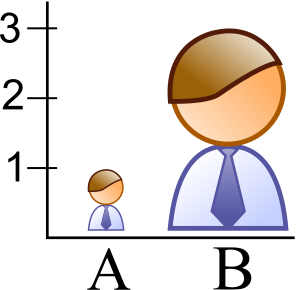
\includegraphics[width=\linewidth]{external/pictograph_scaled.svg}
\end{image}%
%
\par\smallskip%
\noindent\textbf{\blocktitlefont Solution}.\hypertarget{g:solution:idp1542710280}{}\quad{}Though B is 3x taller than A, it is also 3x wider, giving it the appearance of being 9x larger.%
\end{example}
\begin{example}{}{g:example:idp1542706696}%
Discuss your thoughts about the graphic below with one or two people near you.  What do you notice?  What do you believe is missing?%
\par
\begin{image}{0.25}{0.5}{0.25}%
\includegraphics[width=\linewidth]{external/fl_gun_deaths.jpg}
\end{image}%
%
\par\smallskip%
\noindent\textbf{\blocktitlefont Solution}.\hypertarget{g:solution:idp1542711048}{}\quad{}Answers vary, but note that the y-axis is inverted%
\end{example}
\begin{example}{}{g:example:idp1542706312}%
The graph below shows the total amount of debt (in trillions) held by the US government between January and July 2020.%
\par
\begin{image}{0}{1}{0}%
\resizebox{\linewidth}{!}{%
\begin{tikzpicture}
    \begin{axis}[
        title = Total Public Debt (in trillions),
        xmin =0,
        ymin = 22, ymax = 27,
        xtick = {1,2,3,4,5,6,7},
        xticklabels = {Jan,Feb,Mar,Apr,May,Jun,July}
    ]
        \addplot[smooth, mark = *] plot coordinates {(1, 23.2) (2, 23.2) (3, 23.4) (4, 23.7) (5, 24.9) (6, 25.8) (7, 26.4)};
    
    \end{axis}
\end{tikzpicture}
}%
\end{image}%
%
\par
Do you think that the graph gives an accurate picture of the rise of national debt?  Why or why not?%
\par\smallskip%
\noindent\textbf{\blocktitlefont Solution}.\hypertarget{g:solution:idp1542711432}{}\quad{}Answers vary, but generally no.  The data is cherry picked to show only a large jump between April and June 2020 but ignores trends before and after the time range (which are actually fairly stable)%
\end{example}
\end{subsectionptx}
\end{sectionptx}
%
%
\typeout{************************************************}
\typeout{Section 1.4 Measurement \& Units}
\typeout{************************************************}
%
\begin{sectionptx}{Measurement \& Units}{}{Measurement \& Units}{}{}{x:section:data-measurement}
%
%
\typeout{************************************************}
\typeout{Subsection 1.4.1 Measuring Distance}
\typeout{************************************************}
%
\begin{subsectionptx}{Measuring Distance}{}{Measuring Distance}{}{}{x:subsection:data-measurement-distance}
There are many ways of measuring distance.  Here are a few common units of measurement for distance.%
\par
%
\begin{itemize}[label=\textbullet]
\item{}Inches (in)%
\item{}Feet (ft)%
\item{}Yards (yd)%
\item{}Miles (mi)%
\item{}Centimeters (cm)%
\item{}Meters (m)%
\item{}Kilometers (km)%
\end{itemize}
%
\begin{example}{}{g:example:idp1542714632}%
Give an example of something that can be measured using each of the units above.%
\par\smallskip%
\noindent\textbf{\blocktitlefont Solution}.\hypertarget{g:solution:idp1542718216}{}\quad{}Answers vary%
\end{example}
\begin{assemblage}{Relationships Between Units.}{g:assemblage:idp1542715400}%
%
\begin{itemize}[label=\textbullet]
\item{}There are 12 inches in 1 foot%
\item{}There are 3 feet in 1 yard%
\item{}There are 5280 feet in 1 mile%
\item{}There are 100 centimeters in 1 meter%
\item{}There are 100 meters in 1 kilometer%
\end{itemize}
%
\end{assemblage}
\begin{example}{}{g:example:idp1542720136}%
Determine an appropriate unit to measure the distance given below.%
\par
%
\begin{enumerate}[label=\alph*]
\item{}Distance between Norman and Oklahoma City%
\item{}Height of a tall building%
\item{}Diameter of a cookie%
\item{}Length of a bug%
\end{enumerate}
%
\par\smallskip%
\noindent\textbf{\blocktitlefont Solution}.\hypertarget{g:solution:idp1542724232}{}\quad{}%
\begin{enumerate}[label=\alph*]
\item{}Miles\slash{}kilometers%
\item{}Feet\slash{}meters%
\item{}Inches\slash{}centimeters%
\item{}Inches\slash{}centimeters%
\end{enumerate}
%
\end{example}
Converting between units is very important to help us conceptualize and compute information.%
\begin{example}{}{g:example:idp1542734088}%
If there are 3.28 feet in 1 meter, convert 1 mile to 1 kilometer%
\par\smallskip%
\noindent\textbf{\blocktitlefont Solution}.\hypertarget{g:solution:idp1542729352}{}\quad{}1 mile is 1.61 km%
\end{example}
\begin{example}{}{g:example:idp1542733576}%
Convert your height from imperial units (feet and inches) to centimeters.  Use the fact that there are 2.54 centimeters in 1 inch.%
\par\smallskip%
\noindent\textbf{\blocktitlefont Solution}.\hypertarget{g:solution:idp1542734216}{}\quad{}Answers vary%
\end{example}
\begin{example}{}{g:example:idp1542733704}%
Example about converting distances in space%
\par\smallskip%
\noindent\textbf{\blocktitlefont Solution}.\hypertarget{g:solution:idp1542728968}{}\quad{}%
\end{example}
\end{subsectionptx}
%
%
\typeout{************************************************}
\typeout{Subsection 1.4.2 Measuring Area}
\typeout{************************************************}
%
\begin{subsectionptx}{Measuring Area}{}{Measuring Area}{}{}{x:subsection:data-measurement-area}
While length measures one dimensional objects, area is a measure of two-dimensional objects.%
\begin{assemblage}{Area Formulas for Common Shapes.}{g:assemblage:idp1542729736}%
%
\begin{itemize}[label=\textbullet]
\item{}Rectangles: Length\(\cdot\) Width%
\item{}Triangles: \(\dfrac{1}{2}\cdot\) Length \(\cdot\) Width%
\item{}Circles: \(\pi\cdot\)Radius\(^2\)%
\end{itemize}
%
\end{assemblage}
The units of area are similar to the units of length; we find the units for area by squaring the component length unit.  Some common area units are:%
\par
%
\begin{itemize}[label=\textbullet]
\item{}square inches (in\(^2\))%
\item{}square miles (mi\(^2\))%
\item{}square meters (m\(^2\))%
\end{itemize}
%
\begin{example}{}{g:example:idp1542741512}%
Give an example of something that could be measured using each of the units above%
\par\smallskip%
\noindent\textbf{\blocktitlefont Solution}.\hypertarget{g:solution:idp1542738440}{}\quad{}Answers vary%
\end{example}
\begin{example}{}{g:example:idp1542741640}%
A new house has a 2.5 acre lot.  What is the square footage of the lot?  Use the fact that there are 3 feet in 1 yard, and 4,840 square yards in 1 acre.%
\par\smallskip%
\noindent\textbf{\blocktitlefont Solution}.\hypertarget{g:solution:idp1542739592}{}\quad{}108,900 square feet%
\end{example}
\end{subsectionptx}
%
%
\typeout{************************************************}
\typeout{Subsection 1.4.3 Measuring Volume}
\typeout{************************************************}
%
\begin{subsectionptx}{Measuring Volume}{}{Measuring Volume}{}{}{x:subsection:data-measurement-volume}
Volume is a measure of three-dimensional objects, the three-dimensional analogue of area.%
\begin{assemblage}{Volume Formulas for Common Shapes.}{g:assemblage:idp1542749448}%
%
\begin{itemize}[label=\textbullet]
\item{}Rectangular prism: Length\(\cdot\)Width\(\cdot\)Height%
\item{}Sphere: \(\dfrac{4\pi}{3}\cdot\)Radius\(^3\)%
\end{itemize}
%
\end{assemblage}
\begin{example}{}{g:example:idp1542746760}%
A new piece of luggage has a carrying capacity of 5.2 cubic feet of storage space.  How many cubic inches of space is there?%
\par\smallskip%
\noindent\textbf{\blocktitlefont Solution}.\hypertarget{g:solution:idp1542751112}{}\quad{}There are 8985.6 cubic inches of space.%
\end{example}
Liquid volume is often measured with special units.  Some of these are:%
\par
%
\begin{itemize}[label=\textbullet]
\item{}Milliliters (mL)%
\item{}Liters (L)%
\item{}Fluid Ounces (oz)%
\item{}Cups (c)%
\item{}Quarts (qt)%
\item{}Gallons (gal)%
\end{itemize}
%
\begin{assemblage}{Relationships Between Units.}{g:assemblage:idp1542759560}%
%
\begin{itemize}[label=\textbullet]
\item{}There are 1000 milliliters in 1 liter%
\item{}There are 8 fluid ounces in 1 cup%
\item{}There are 4 cups in 1 quart%
\item{}There are 4 quarts in 1 gallon%
\end{itemize}
%
\end{assemblage}
\begin{example}{}{g:example:idp1542758792}%
How many fluid ounces are in 2 gallons?%
\par\smallskip%
\noindent\textbf{\blocktitlefont Solution}.\hypertarget{g:solution:idp1542757768}{}\quad{}256 fluid ounces are in 1 gallon%
\end{example}
\end{subsectionptx}
%
%
\typeout{************************************************}
\typeout{Subsection 1.4.4 Measuring Temperature}
\typeout{************************************************}
%
\begin{subsectionptx}{Measuring Temperature}{}{Measuring Temperature}{}{}{x:subsection:data-measurement-temperature}
There are two primary units used to measure temperature: Fahrenheit and Celsius%
\begin{assemblage}{Converting Between Fahrenheit and Celsius.}{g:assemblage:idp1542756872}%
To convert from Fahrenheit to Celsius, use the formula%
\begin{equation*}
^\circ C = (^\circ F-32)\cdot \dfrac{5}{9}
\end{equation*}
%
\par
To convert from Celsius to Fahrenheit, use the formula%
\begin{equation*}
^\circ F = ^\circ C\cdot \dfrac{9}{5} + 32
\end{equation*}
%
\par
A decent estimate to go from Celsius to Fahrenheit is to double the Celsius temperature, then add 32.%
\end{assemblage}
\begin{example}{}{g:example:idp1542765704}%
The average high in Norman in October is 75\(^\circ F\).  How high is that in Celsius?%
\par\smallskip%
\noindent\textbf{\blocktitlefont Solution}.\hypertarget{g:solution:idp1542765064}{}\quad{}About 23.9\(^\circ C\)%
\end{example}
\begin{example}{}{g:example:idp1542761096}%
The 2022 Men's World Cup was moved from Summer 2022 to Winter 2022 because the average temperature in Qatar is about 41\(^\circ C\).  About how hot is that in Fahrenheit?%
\par\smallskip%
\noindent\textbf{\blocktitlefont Solution}.\hypertarget{g:solution:idp1542761224}{}\quad{}About 114\(^\circ F\)%
\end{example}
\end{subsectionptx}
\end{sectionptx}
%
%
\typeout{************************************************}
\typeout{Section 1.5 Ratios, Rates, Proportions}
\typeout{************************************************}
%
\begin{sectionptx}{Ratios, Rates, Proportions}{}{Ratios, Rates, Proportions}{}{}{x:section:data-rrp}
%
%
\typeout{************************************************}
\typeout{Subsection 1.5.1 Rates \& Ratios}
\typeout{************************************************}
%
\begin{subsectionptx}{Rates \& Ratios}{}{Rates \& Ratios}{}{}{x:subsection:data-rrp-rate}
\begin{definition}{}{x:definition:ratio}%
A \terminology{ratio} is a comparison of amounts or quantities.%
\index{Ratio}%
\end{definition}
\begin{example}{}{g:example:idp1542764424}%
The Dodge Family College of Arts and Sciences oversees 30 departments while the Gallogly College of Engineering has 9 departments.  What is the ratio of Arts and Sciences departments to Engineering departments?%
\par\smallskip%
\noindent\textbf{\blocktitlefont Solution}.\hypertarget{g:solution:idp1542771208}{}\quad{}10\slash{}3%
\end{example}
Ratios can be expressed several ways%
\begin{assemblage}{Ratio Expressions.}{g:assemblage:idp1542770056}%
%
\begin{itemize}[label=\textbullet]
\item{}Simplified fractions in the form \(\dfrac{a}{b}\)%
\item{}With a colon in the form \(a:b\)%
\item{}Verbally in the form "\(a\) to \(b\)"%
\end{itemize}
%
\end{assemblage}
\begin{example}{}{g:example:idp1542867656}%
Express the answer from the previous example in two other ways%
\par\smallskip%
\noindent\textbf{\blocktitlefont Solution}.\hypertarget{g:solution:idp1542869320}{}\quad{}\(10:3\) or 10 to 3%
\end{example}
\begin{example}{}{g:example:idp1542867400}%
What is the ratio of glasses-wearing students to non-glasses-wearing students in the class?%
\par\smallskip%
\noindent\textbf{\blocktitlefont Solution}.\hypertarget{g:solution:idp1542866760}{}\quad{}Answers vary%
\end{example}
\begin{example}{}{g:example:idp1542871368}%
In Giada de Laurentiis' recipe for lasagna rolls, she calls for 15 ounces of ricotta and 1 cup of shredded mozzarella cheese.  What is the ratio of mozzarella to ricotta?  1 dry cup is equal to 6.8 ounces.%
\par\smallskip%
\noindent\textbf{\blocktitlefont Solution}.\hypertarget{g:solution:idp1542866632}{}\quad{}6.8:15%
\end{example}
\begin{definition}{}{x:definition:rate}%
A \terminology{rate} is a ratio comparing two items with different units%
\index{Rate}%
\end{definition}
\begin{example}{}{g:example:idp1542871240}%
Give five different examples of rates that you might see in the wild.%
\par\smallskip%
\noindent\textbf{\blocktitlefont Solution}.\hypertarget{g:solution:idp1542867784}{}\quad{}Answers vary%
\end{example}
\begin{example}{}{g:example:idp1542878152}%
On March 16, 2022, Shai Gilgeous-Alexander scored 14 field goals on 22 shot attempts against the San Antonio Spurs.%
\par
%
\begin{enumerate}[label=\alph*]
\item{}What is the rate of field goals made to field goals attempted?%
\item{}When we perform the division represented by a rate, we find the \terminology{unit rate}.  What was Gilgeous-Alexander's unit rate for shots attempted to shots made in this game?  (In basketball, this unit rate is called the field goal percentage)%
\end{enumerate}
%
\par\smallskip%
\noindent\textbf{\blocktitlefont Solution}.\hypertarget{g:solution:idp1542882632}{}\quad{}%
\begin{enumerate}[label=\alph*]
\item{}7:11%
\item{}0.636%
\end{enumerate}
%
\end{example}
\begin{example}{}{g:example:idp1542879176}%
According to Google Maps, the distance between Oklahoma State and the University of Oklahoma is 88.1 miles.  Amy drove from OSU to OU in exactly 100 minutes.  What the unit rate (in miles per hour) for her speed on the trip? (This unit rate is her average speed)%
\par\smallskip%
\noindent\textbf{\blocktitlefont Solution}.\hypertarget{g:solution:idp1542881736}{}\quad{}52.8 miles per hour%
\end{example}
\begin{example}{}{g:example:idp1542875848}%
At Walmart, a 12.4 oz box of Cheez-Its costs \textdollar{}3.68 while a 21 oz box costs \textdollar{}5.28.  Which box is the most cost effective purchase?  Why?%
\par\smallskip%
\noindent\textbf{\blocktitlefont Solution}.\hypertarget{g:solution:idp1542879560}{}\quad{}The 21 oz box cost 25.1 cents per ounce while the 12.4 oz box costs 29.7 cents per ounce; thus, the larger box is more cost effective.%
\end{example}
\end{subsectionptx}
%
%
\typeout{************************************************}
\typeout{Subsection 1.5.2 Proportions}
\typeout{************************************************}
%
\begin{subsectionptx}{Proportions}{}{Proportions}{}{}{x:subsection:data-rrp-prop}
\begin{definition}{}{x:definition:proportion}%
A \terminology{proportion} is an equation which relates two ratios.%
\index{Proportion}%
\end{definition}
\begin{example}{}{g:example:idp1542886088}%
Write a proportion relating the number of centimeters in one meter to the number of centimeters in five meters.%
\par\smallskip%
\noindent\textbf{\blocktitlefont Solution}.\hypertarget{g:solution:idp1542889032}{}\quad{}\(\dfrac{100\text{ cm}}{1\text{ m}} = \dfrac{500\text{ cm}}{5\text{ m}}\)%
\end{example}
\begin{example}{}{g:example:idp1542887368}%
Is the proportion \(\dfrac{5}{8} = \dfrac{55}{80}\) true or false?  Why?%
\par\smallskip%
\noindent\textbf{\blocktitlefont Solution}.\hypertarget{g:solution:idp1542885576}{}\quad{}False, since the numbers aren't equivalent.  Cross multiplying is probably the easiest way of seeing this.%
\end{example}
\begin{example}{}{g:example:idp1542888648}%
25\% of what number is 32?%
\par\smallskip%
\noindent\textbf{\blocktitlefont Solution}.\hypertarget{g:solution:idp1542889416}{}\quad{}128%
\end{example}
\begin{example}{}{g:example:idp1542890824}%
You have an irregularly sized photograph measuring 4 inches by 8 inches, but want to scale it up so that the larger side measures 20 inches.  How long does the shorter side have to be to maintain the size ratio?%
\par\smallskip%
\noindent\textbf{\blocktitlefont Solution}.\hypertarget{g:solution:idp1542883272}{}\quad{}10 inches%
\end{example}
\end{subsectionptx}
\end{sectionptx}
\end{chapterptx}
\end{document}